\subsection{The Star Formation Rate Distribution Function}
\label{sec:cos_sfrf}

\begin{figure}
	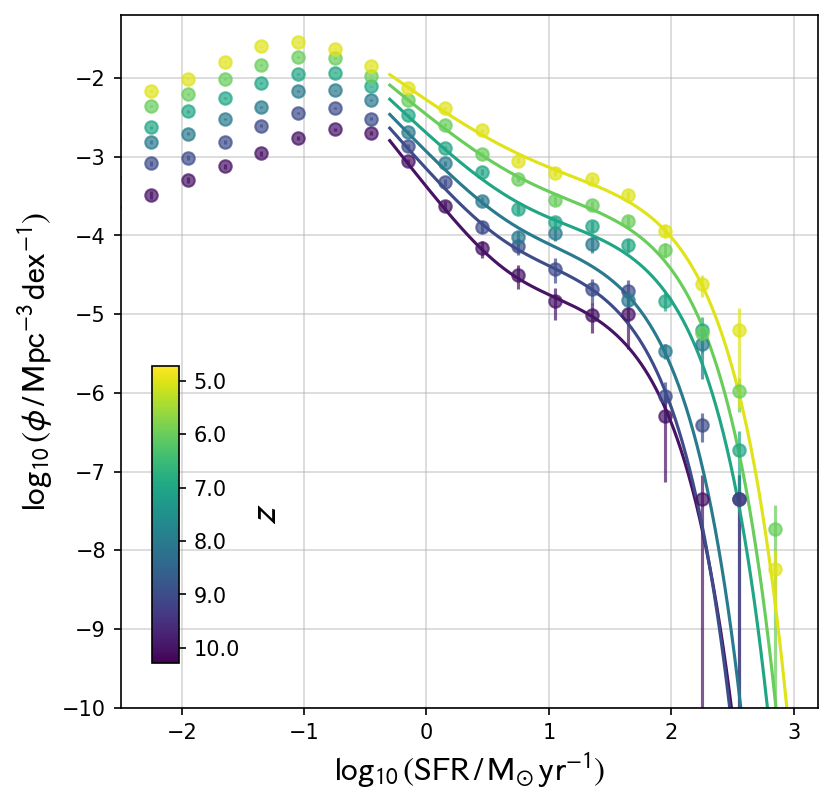
\includegraphics[width=\columnwidth]{images/sfrf_all.png}
    \caption{Redshift evolution of the \flares\ composite star formation rate distribution function.
		Points show binned differential counts with Poisson 1$\sigma$ uncertainties from the simulated number counts.
		Solid lines show double-Schechter function fits, quoted in \tab{sfrf_schechter_params}.}
    \label{fig:sfrf_all}
\end{figure}

The Star Formation Rate distribution Function (SFRF) describes the number of galaxies per unit volume per unit star formation rate interval d$\log_{10}\SFR$, where $\SFR$ is the star formation rate,
\begin{align}
     \phi(\SFR) = N \,/\, \mathrm{Mpc^{-3} \, dex^{-1}}\;\;.
\end{align}
We define the SFR as the sum of the instantaneous SFR of all star forming gas particles within a 30 kpc aperture centred on the potential minimum of the subhalo.

\subsubsection{The cosmic SFRF}
\label{sec:results:sfrf:cosmic}

In \fig{sfrf_all} we plot the evolution of the \flares\ composite SFRF.
We provide counts in bins 0.3 dex in width.
There is a clear low-mass turnover between $\sim 0.1\,-\,0.5 \, \mathrm{M_{\odot} \; yr^{-1}}$, but above this the shape is well described by a double-Schechter function.
We provide fits using the following parametrisation,
\begin{align}
    \phi(\SFR) \, \mathrm{d}\log_{10}&\SFR = \mathrm{ln}(10) \, e^{-\SFR/\SFR^*} \times \nonumber\\
    & \left[ \, \phi^{*}_{1} \, \left(\frac{\SFR}{\SFR^*} \right)^{\alpha_{1} + 1} + \phi^{*}_{2} \, \left(\frac{\SFR}{\SFR^*} \right)^{\alpha_{2} + 1} \right].
\end{align}
We limit our fits to those galaxies with $\SFR > 1 \, \mathrm{M_{\odot} \; yr^{-1}}$; these fits are provided in \tab{sfrf_schechter_params}.
We also plot the parameter evolution with redshift in \Fig{fit_param_evolution}.
The characteristic star formation rate, $\SFR_*$, is offset by $+10^{8}$ to aid comparison with the GSMF characteristic mass, $\mathrm{M_{*}}$.

The normalisation of both components ($\phi_{1};\,\phi_{2}$), as well as the low-SFR slope ($\alpha_{1}$), increase with decreasing redshift.
These trends are surprisingly similar to those seen for the equivalent parameters in the GSMF.
The low-SFR normalisation is almost identical, as is the high-SFR normalisation, with a small $\sim +0.2\;\mathrm{dex}$ offset.
The low-SFR slope $\alpha_1$ is shallower than that of the GSMF at the highest redshifts ($z\geqslant 8$), but identical at lower redshifts.
However, the evolution of the characteristic SFR is significantly flatter compared to that of the characteristic mass for the GSMF.
This suggests a redshift-independent upper limit to the SFR.

\begin{figure*}
	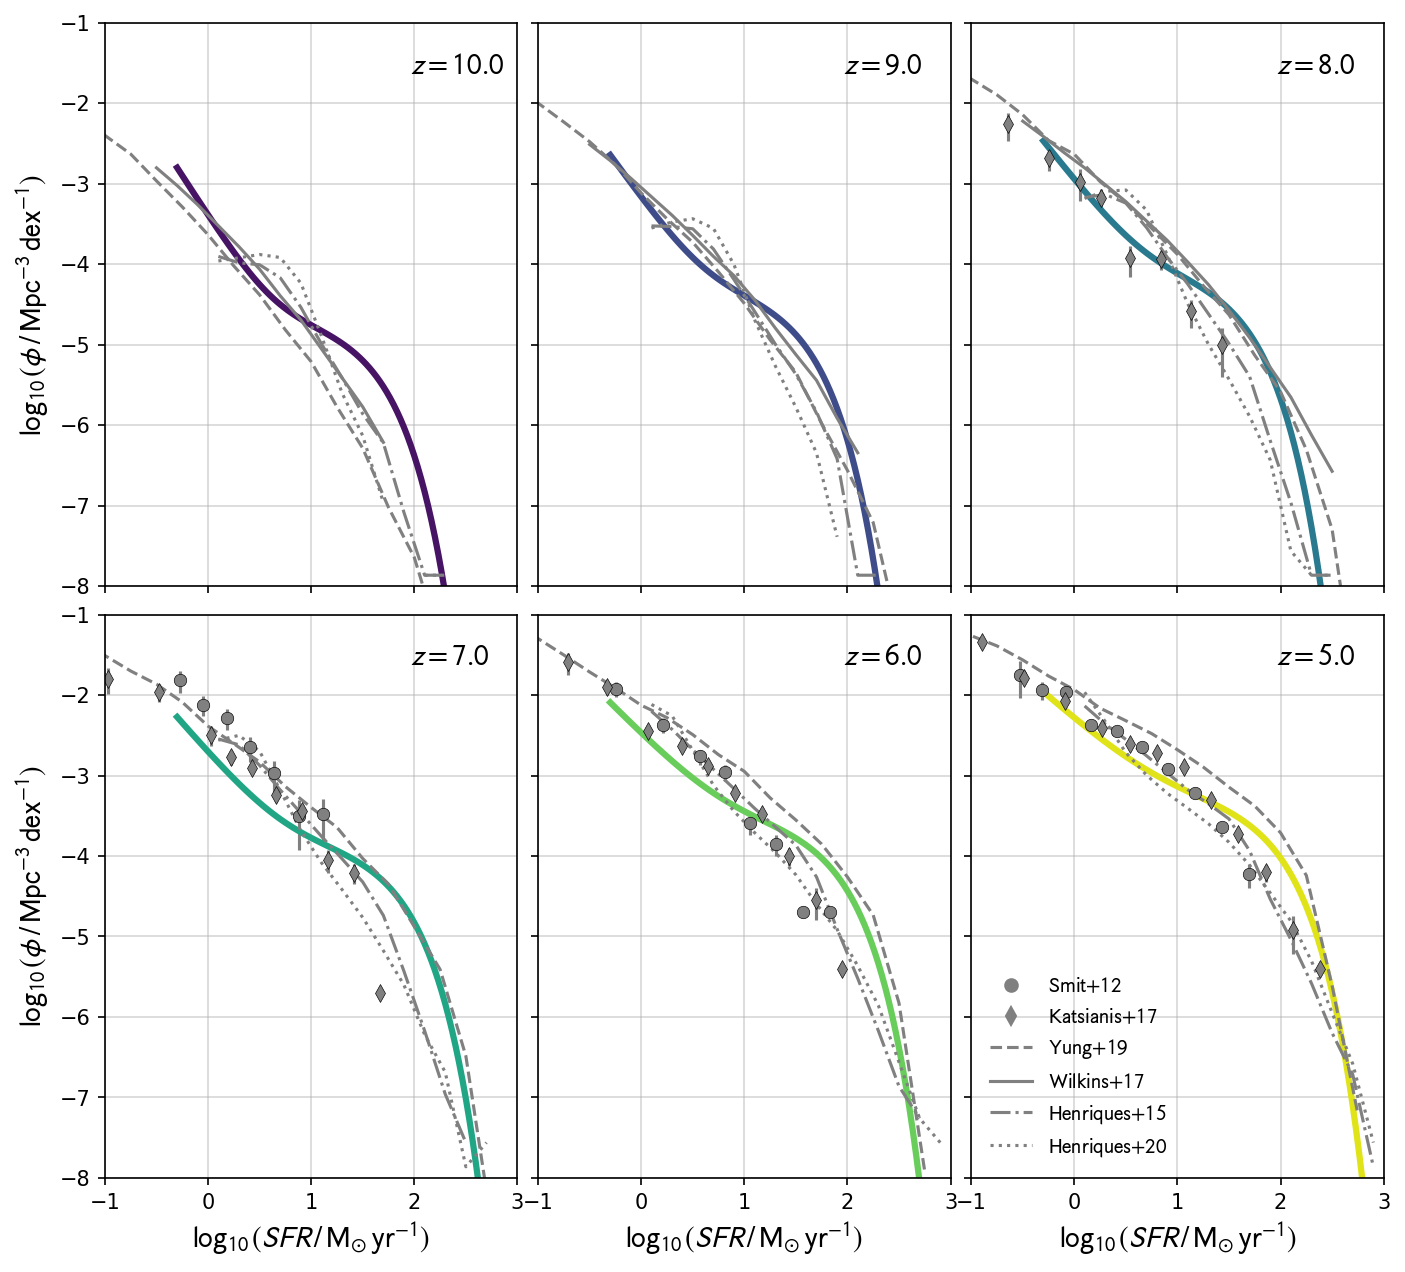
\includegraphics[width=\textwidth]{images/sfrf_multi_both.png}
        \caption{Evolution of the \flares\ composite star formation rate distribution function (coloured, solid lines), compared with observational constraints from UV data and other model predictions.
				\protect\cite{smit_star_2012} derive SFRs from UVLF data, as do \protect\cite{katsianis_evolution_2017} using \protect\cite{bouwens_uv_2015} data.
				Both are corrected to a Chabrier IMF using the conversion factors quoted in \protect\cite{kennicutt_jr_star_2012}.
				The Santa-Cruz SAM \protect\citep[][dashed line]{yung_semi-analytic_2019} and \bluetides\ simulation \protect\citep{wilkins_properties_2017} show a different behaviour, with a power law shape at higher redshifts, in contrast to the prominent knee seen in \flares\ up to $z = 10$.
				Both \lgals\ models also show similar behaviour, though with lower normalisation at the high-SFR end \citep{henriques_galaxy_2015,henriques_l-galaxies_2020}.
				}
        \label{fig:sfrf_multi_both}
\end{figure*}


This double-Schechter form of the SFRF is in some tension with observational constraints.
\fig{sfrf_multi_both} shows a comparison with UV derived relations from \cite{smit_star_2012} and \cite{katsianis_evolution_2017} (the latter using \citealt{bouwens_uv_2015} data).
For low-SFRs the observed normalisation is slightly higher ($\sim \, 0.3$ dex) from $z = 5$ to $7$.
There is no prominent knee in the observed relations, and the exponential tail drops off at lower SFRs than in the simulations.

\fig{sfrf_multi_both} also shows results from recent cosmological models.
As with the GSMF, there is some tension with the SFRF produced by the Santa Cruz models \citep{yung_semi-analytic_2019}.
\flares\ has a distinct double-Schechter shape, whereas the SC model appears as a single schechter at $z = 5$, before evolving to a power law at $z = 10$.
The \bluetides\ results \citep{wilkins_properties_2017} also show a similar power law relation at $z \geqslant 8$, in tension with the prominent knee in \flares.
Both \lgals\ models show similar power law-like behaviour, though with lower normalisation at the high-SFR end \citep{henriques_galaxy_2015,henriques_l-galaxies_2020}, though in better agreement with the existing observational data at $z = 6$ compared to the Santa Cruz model and \flares.

The offset in normalisation of the \flares\ SFRF at high SFRs with the observations may be a selection effect due to highly dust-obscured galaxies.
These galaxies, with number densities of $\sim 10^{-5} \; \mathrm{cMpc^{-3}}$  at $z \sim 2$ \citep{simpson_alma_2014}, will be missed in higher redshift rest frame-UV observations.
We will perform a direct comparison with the UV luminosity function, including selfconsistent modelling of dust attentuation, in Paper II, Vijaiyan et al. (2020,\textit{in prep.}).

To investigate what effect our sampling of highly overdense regions has on the composite shape of the SFRF, we now look at the overdensity dependence of the SFRF.

% \peter{why? - perhaps to do with our much better sampling of rare peaks -- the mean density regioni in Fig 11 looks much more like a power law.}

\subsubsection{Environmental dependence of the SFRF}
\label{sec:env_sfrf}

\begin{figure}
	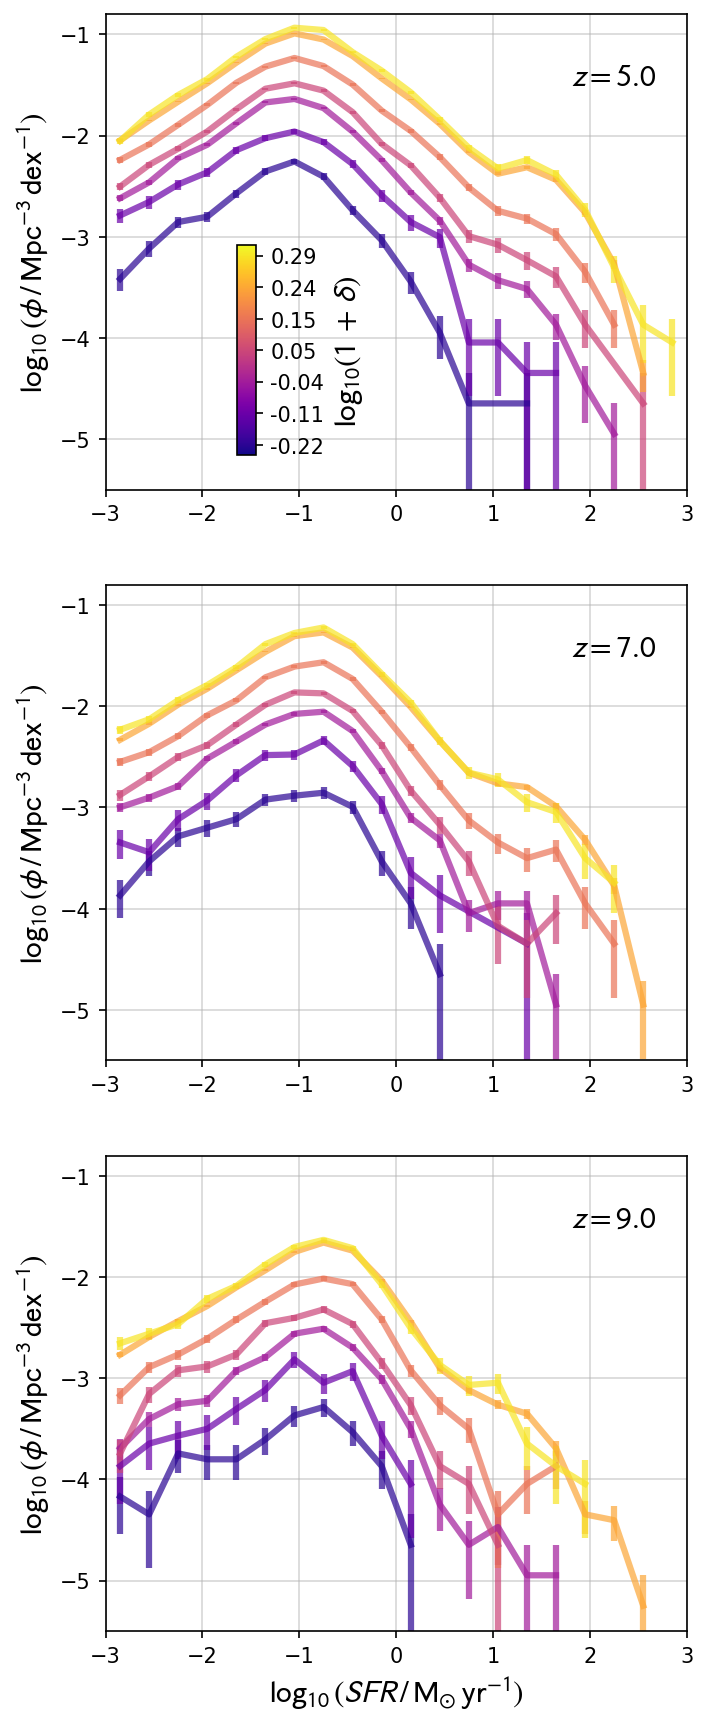
\includegraphics[width=\columnwidth]{images/sfrf_overdensity.png}
    \caption{The \flares\ SFRF between $z = 5$ and $9$ split by binned log-overdensity.
		Poisson 1$\sigma$ uncertainties are shown for each bin from the simulated number counts.
		The normalisation increases with increasing overdensity, and the maximum SFR increases.}
    \label{fig:sfrf_overdensity}
\end{figure}

\fig{sfrf_overdensity} shows the SFRF for regions binned by their log-overdensity.
There is almost no variation in the shape as a function of overdensity except for the highest overdensities, which show a more prominent double-Schechter knee in the high-SFR regime.
This behaviour is identical to that seen for the GSMF.
This may explain why the shape of the \flares\ composite SFRF differs with those of other cosmological models.
\flares\ better samples the rare, high-density regions that contribute significantly to the high-SFR ($\SFR > 100 \, \mathrm{M_{\odot} yr^{-1}}$) tail of the SFRF.
Both \bluetides\ and the Santa-Cruz model are run on regions with much smaller volumes ($500^{3}$ and $357^{3}$ $\mathrm{cMpc^3}$, respectively), which may not probe the extreme regions sampled in the \flares\ parent volume.
The mean density region in \fig{sfrf_overdensity} appears power law-like at all redshifts, which may present a better comparison with these models.


As for the GSMF, we provide fits to the normalisation at a given SFR and redshift, in the following form,
\begin{equation}
  \phi \,(\mathrm{log_{10}}(1+\delta) \,|\, \SFR, z) = m \,[\mathrm{log_{10}}(1+\delta)] + c,
\end{equation}
where $\mathrm{log_{10}}(1\,+\,\delta)$ is the overdensity of the region.
\tab{norm_SFRF} shows these fits for bins $\pm 0.2$ \; dex wide centred at $\mathrm{log_{10}(\SFR\,/\,M_{\odot} \, yr^{-1})} = [-0.5,\,0.5]$.
% \peter{Once again, what is the purpose of this table? -- that's not a rhetorical question.}
The normalisation increases with increasing overdensity as expected.
The trends with redshift are also broadly similar to those seen for the GSMF.
\footnote{The only exception being the gradient of the GSMF relation at $M_{*} \,/\,M_{\odot} = 10^{9.7}$, which decreases with redshift,  whereas the redshift dependence is positive for the SFRF at all SFRs.}


\begin{table}
	\centering
	\caption{Fits to the normalisation, $\log_{10}(\phi_\SFR/\mathrm{Mpc^{-3} \, dex^{-1}}$) of the SFRF at different redshifts and star formation rates (see \protect\sec{env_sfrf}).}
	\label{tab:norm_SFRF}
	\begin{tabular}{lccc} % four columns, alignment for each
		\hline
		$z$ & $\log_{10}(\SFR \,/\, \Msun \, \mathrm{yr}^{-1})$ & $m$ & $c$ \\
		\hline
        5 & -0.5 & 3.0 & -2.0 \\
        7 & -0.5 & 3.2 & -2.2 \\
        9 & -0.5 & 3.5 & -2.6 \\
        5 & 0.5 & 3.8 & -2.8 \\
        7 & 0.5 & 4.4 & -3.4 \\
        9 & 0.5 & 4.5 & -4.0 \\
        \hline
	\end{tabular}
\end{table}
